\documentclass[10pt]{article}
\usepackage[margin=2.2cm]{geometry}
\usepackage{graphicx}\usepackage{booktabs}\usepackage{amsmath}\usepackage{amssymb}
\usepackage{xcolor}\usepackage[hidelinks]{hyperref}
\setlength{\parskip}{4pt}\setlength{\parindent}{0pt}
\graphicspath{{../../../output/04_axicon/}}
\title{\vspace{-1.2cm}\textbf{Review 04 --- Axicon / Bessel beams}\\
\large \texttt{mcdo\_dev} Phase 4 \quad(\texttt{output/04\_axicon/},
\texttt{docs/theory/04\_axicon.md})}
\author{}\date{2026-06-13}
\begin{document}\maketitle\vspace{-1.1cm}

\section*{Construction}
Conical pupil phase $A(\theta)=\exp(+j\beta\sin\theta/\sin\alpha)$ (true axicon:
phase $\propto$ pupil radius). Stationary phase maps axial position to cone
angle, $u(\theta^{*})=\beta\sin\alpha\cot\theta^{*}$, with local transverse profile
$J_0^2(v\sin\theta^{*}/\sin\alpha)$ [Durnin 1987]. Linear-$x$ y-cut.

\begin{itemize}\itemsep1pt
\item $\beta=0$ regression $\equiv$ plain disk: max diff 0 (exact).
\item Focal segment forms at $u>0$, onset $u\approx\beta\cos\alpha$; bright
  length 10.9 / 14.2 / 17.9 for $\beta$=10/20/40 (plain focus FWHM 9.9).
\item \textbf{Durnin checkpoint}: at $\theta^{*}$=0.55/0.70/0.85$\alpha$ the
  transverse profile at the predicted $u$ matches $J_0^2(v\sin\theta^{*}/\sin\alpha)$
  to max dev \textbf{0.04--0.08}, at both $X_{NA}$=0.13 and 0.8.
\item Axicon local profile $\equiv$ thin annulus at the matched $\theta$ ---
  two roads to one Bessel core.
\end{itemize}

\textbf{Flag (honest):} the 0.04--0.08 $J_0^2$ deviation is \emph{comparable
at low and high NA}, so it is the stationary-phase-approximation error
(finite segment + amplitude taper), \emph{not} a vector effect. The clean
vector-Bessel probe is the thin annulus (Phase 3: dev 0.163 at sin$\alpha$=0.9
vs 0.004 low NA). The axicon's DOF gain ($\sim$1.4--1.8$\times$) is modest next
to the annulus ($\sim$44$\times$); its value is the position-tunable Bessel scale.

\begin{center}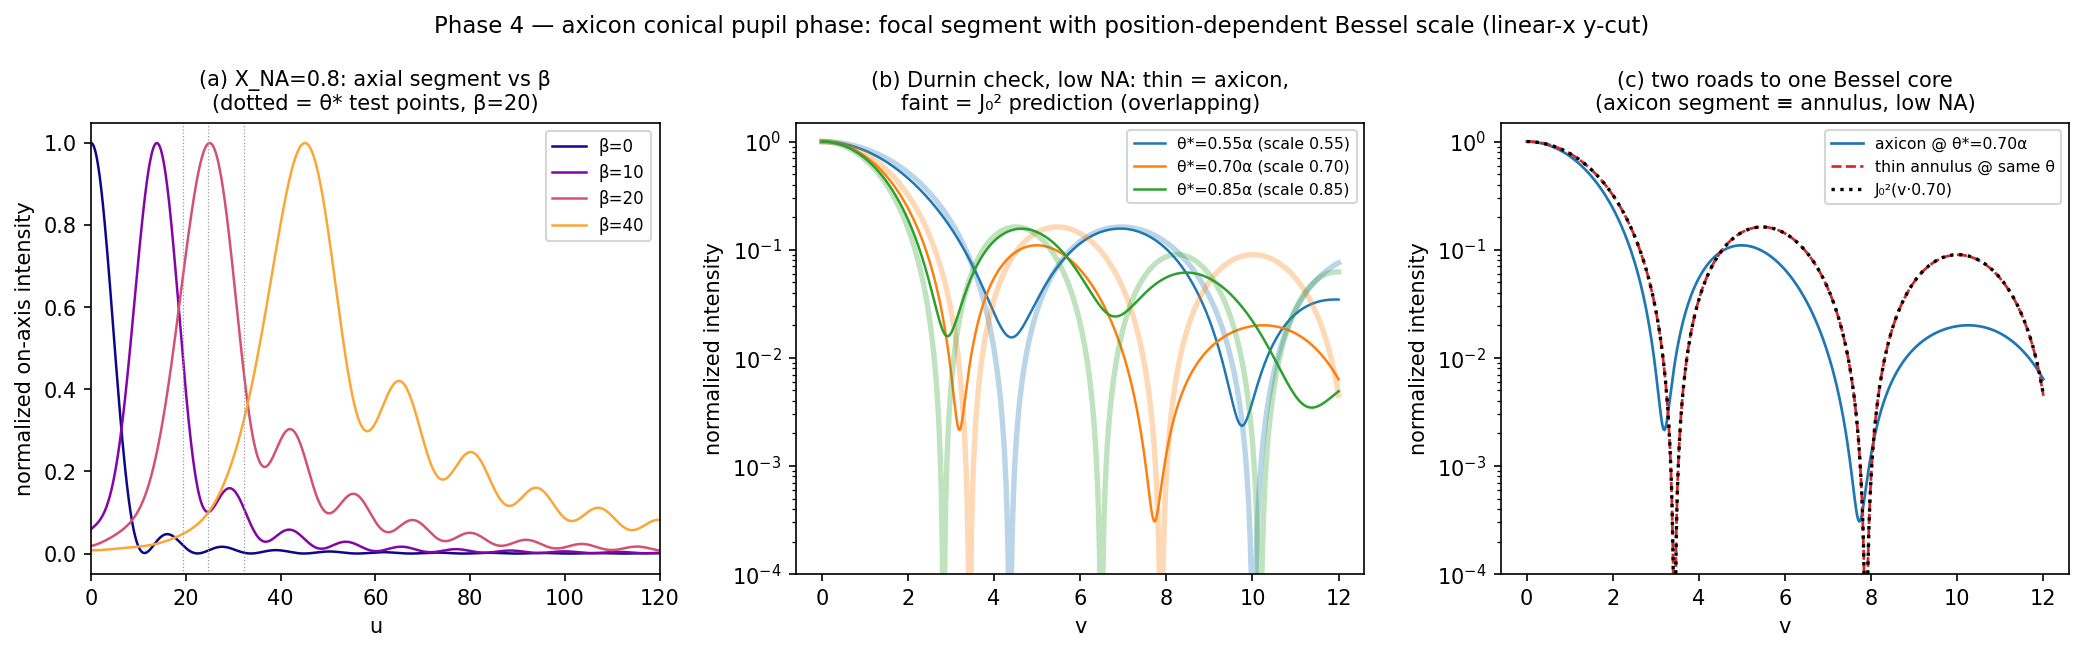
\includegraphics[width=0.99\textwidth]{verify_axicon.png}\end{center}
\textbf{(a)} axial segment vs $\beta$ (dotted = $\theta^{*}$ test points);
\textbf{(b)} low-NA Durnin check (thin = axicon, faint thick = $J_0^2$);
\textbf{(c)} axicon $\equiv$ annulus $\equiv J_0^2$ at $\theta^{*}$=0.70$\alpha$.

\section*{Verification --- push N and $\beta$ to the validity boundary
(\texttt{axicon\_validity.png})}
The 4--8\% above is the stationary-phase \emph{model}, not the method:
\begin{itemize}\itemsep1pt
\item \textbf{More photons} ($\beta$=20, NA=0.8): RMS(MC$-$deterministic) falls
  $\propto 1/\sqrt N$ to a floor $\approx 4\times10^{-4}$ at $N=10^6$.
\item \textbf{Push $\beta$} (NA=0.3, scalar regime, $\theta^{*}$=0.7$\alpha$): the
  $J_0^2$ deviation shrinks $0.134\to0.078\,(\beta{=}20)\to0.006\,(\beta{=}2560)$,
  $\approx 1/\beta$ --- confirming SPA; MC vs deterministic stays $\le 0.019$ at
  every $\beta$ (the method is bias-free).
\item \textbf{Validity ceilings:} $N_\theta{=}3001$ resolves the pupil phase to
  $\beta>2560$ (mathematical); for a real objective ($f\approx2$ mm) the focal
  segment $z^{*}\propto\beta$ leaves the focal region (Debye) at $\beta\approx160$
  --- the physical limit binds first.
\end{itemize}
\begin{center}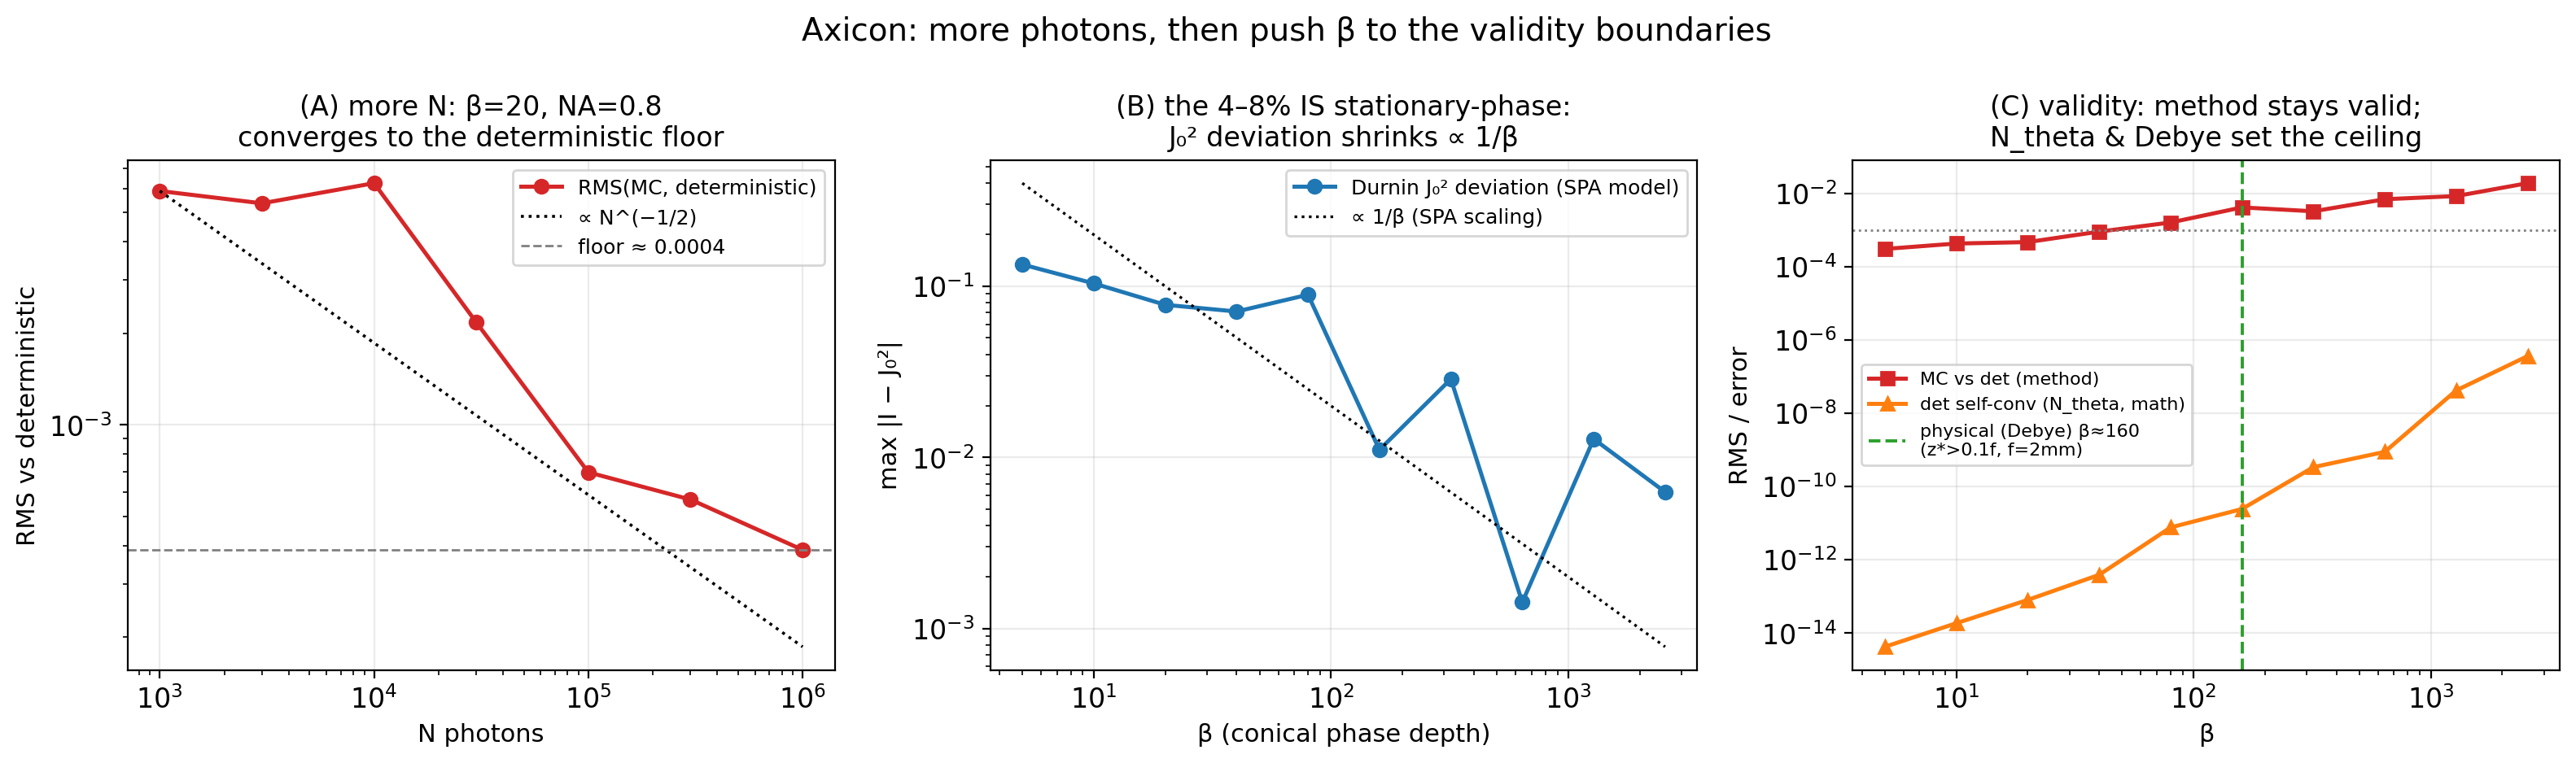
\includegraphics[width=0.99\textwidth]{axicon_validity.png}\end{center}
\textbf{(A)} more N $\to$ deterministic floor; \textbf{(B)} $J_0^2$ deviation
$\propto 1/\beta$ (it IS stationary-phase); \textbf{(C)} method stays valid,
$N_\theta$ \& Debye set the ceiling.
\end{document}
